\chapter{Active Subspace Models}\label{Chap:ActSub}
The idea behind active subspaces is to find directions in the input variable
space in which the quantity of interest is nearly constant. After rotation of
the input variables, this method can allow significant dimension reduction. Below is a brief summary of the process.
\begin{enumerate}
\item Compute the gradient of the quantity of interest, $q = f(\mathbf{x})$,
    at several locations sampled from the full input space,
    $$\nabla_{\mathbf{x}} f_i = \nabla f(\mathbf{x}_i).$$

\item Compute the eigendecomposition of the matrix $\hat{\mathbf{C}}$,
    $$\hat{\mathbf{C}} = \frac{1}{M}\sum_{i=1}^{M}\nabla_{\mathbf{x}} f_i\nabla_{\mathbf{x}} f_i^T = \hat{\mathbf{W}}\hat{\mathbf{\Lambda}}\hat{\mathbf{W}}^T,$$
    where $\hat{\mathbf{W}}$ has eigenvectors as columns, 
    $\hat{\mathbf{\Lambda}} = \text{diag}(\hat{\lambda}_1,\:\ldots\:,\hat{\lambda}_N)$
    contains eigenvalues, and $N$ is the total number of parameters.

\item Using a truncation method or specifying a
    dimension to estimate the active subspace size, 
    split the eigenvectors into active and inactive directions,
    $$\hat{\mathbf{W}} = \left[\hat{\mathbf{W}}_1\quad\hat{\mathbf{W}}_2\right].$$
    These eigenvectors are used to rotate the input variables.

\item Next the input variables, $\mathbf{x}$, are expanded in terms of active and
    inactive variables,
    $$\mathbf{x} = \hat{\mathbf{W}}_1\mathbf{y} + \hat{\mathbf{W}}_2\mathbf{z}.$$

\item A surrogate is then built as a function of the active variables,
    $$g(\mathbf{y}) \approx f(\mathbf{x})$$
\end{enumerate}

As a concrete example, consider the function:~\cite{constantine2015active}
$$f(x) = \exp\left(0.7x_1 + 0.3x_2\right).$$
Figure \ref{fig:activesubspace}(a) is a contour plot of $f(x)$. The black arrows indicate the
eigenvectors of the matrix $\hat{\mathbf{C}}$. Figure \ref{fig:activesubspace}(b) is the same 
function but rotated so that the axes are aligned with the eigenvectors. We arbitrarily
give these rotated axes the labels $y_1$ and $y_2$. From fig.~\ref{fig:activesubspace}(b) it is
clear that all of the variation is along $y_1$ and the dimension of the rotated
input space can be reduced to 1.

\begin{figure}[htbp]
  \begin{subfigmatrix}{2}
  \subfigure[Original function]{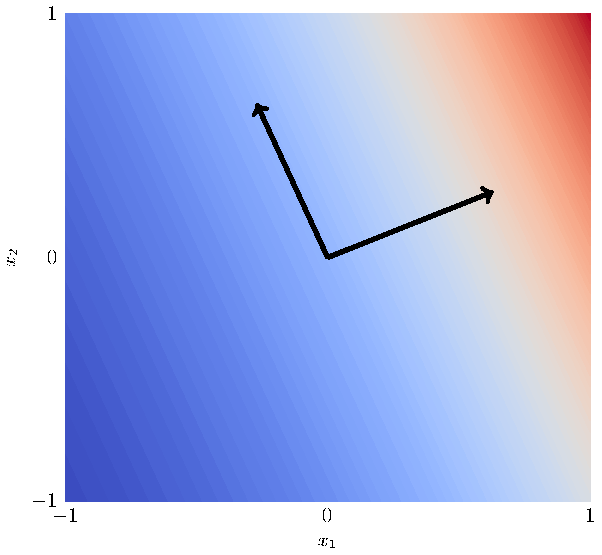
\includegraphics{images/unrotated_example}}
  \subfigure[Rotated function]{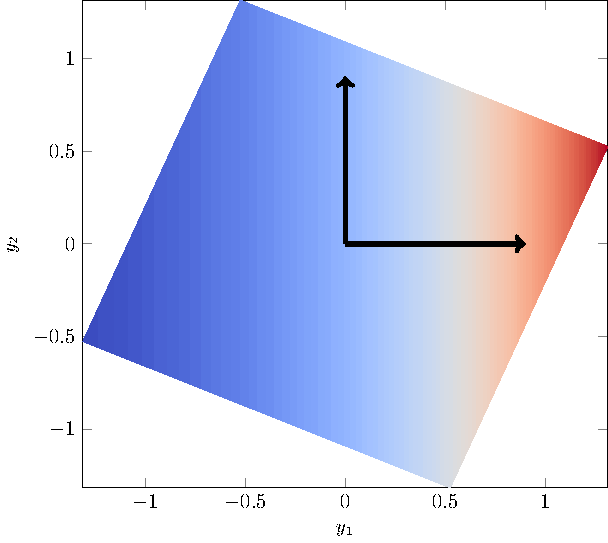
\includegraphics{images/rotated_example}}
  \end{subfigmatrix}
  \caption{Example of a 2D function with a 1D active subspace.}
\label{fig:activesubspace}
\end{figure}

For additional information, see references~\cite{Constantine-preprint-active,constantine2014active,constantine2015active}.

\section{Truncation Methods}\label{Sec:trunc}
Once the eigenvectors of $\hat{\mathbf{C}}$ are obtained we must decide how many
directions to keep. If the exact subspace size is known \textit{a priori} it can be
specified. Otherwise there are three automatic active subspace detection and
truncation methods implemented:
\begin{itemize}
\item Constantine metric (default),
\item Bing Li metric,
\item and Energy metric.
\end{itemize}

\subsection{Constantine metric}\label{SubSec:constantine}
The Constantine metric uses a criterion based on the variability of the subspace estimate. 
Eigenvectors are computed for bootstrap samples of the gradient matrix. The 
subspace size associated with the minimum distance between bootstrap 
eigenvectors and the nominal eigenvectors is the estimated active subspace
size.

Below is a brief outline of the Constantine method of active subspace 
identification. The first two steps are common to all active subspace 
truncation methods.
\begin{enumerate}
\item Compute the gradient of the quantity of interest, $q = f(\mathbf{x})$,
    at several locations sampled from the input space,
    $$\nabla_{\mathbf{x}} f_i = \nabla f(\mathbf{x}_i).$$

\item Compute the eigendecomposition of the matrix $\hat{\mathbf{C}}$,
    $$\hat{\mathbf{C}} = \frac{1}{M}\sum_{i=1}^{M}\nabla_{\mathbf{x}} f_i\nabla_{\mathbf{x}} f_i^T = \hat{\mathbf{W}}\hat{\mathbf{\Lambda}}\hat{\mathbf{W}}^T,$$
    where $\hat{\mathbf{W}}$ has eigenvectors as columns, 
    $\hat{\mathbf{\Lambda}} = \text{diag}(\hat{\lambda}_1,\:\ldots\:,\hat{\lambda}_N)$
    contains eigenvalues, and $N$ is the total number of parameters.

\item Use bootstrap sampling of the gradients found in step 1 to compute replicate
    eigendecompositions,
    $$\hat{\mathbf{C}}_j^* = \hat{\mathbf{W}}_j^*\hat{\mathbf{\Lambda}}_j^*\left(\hat{\mathbf{W}}_j^*\right)^T.$$

\item Compute the average distance between nominal and bootstrap subspaces,
    $$e^*_n = \frac{1}{M_{boot}}\sum_j^{M_{boot}} \text{dist}(\text{ran}(\hat{\mathbf{W}}_n), \text{ran}(\hat{\mathbf{W}}_{j,n}^*)) = \frac{1}{M_{boot}}\sum_j^{M_{boot}} \left\| \hat{\mathbf{W}}_n\hat{\mathbf{W}}_n^T - \hat{\mathbf{W}}_{j,n}^*\left(\hat{\mathbf{W}}_{j,n}^*\right)^T\right\|,$$
    where $M_{boot}$ is the number of bootstrap samples, 
    $\hat{\mathbf{W}}_n$ and $\hat{\mathbf{W}}_{j,n}^*$ both contain 
    only the first $n$ eigenvectors, and $n < N$.

\item The estimated subspace rank, $r$, is then,
    $$r = \operatorname*{arg\,min}_n \, e^*_n.$$
\end{enumerate}

For additional information, see Ref.~\cite{constantine2015active}.

\subsection{Bing Li metric}\label{SubSec:bingli}
The Bing Li metric uses a trade-off criterion to determine where to truncate the active subspace.
The criterion is a function of the eigenvalues
and eigenvectors of the active subspace gradient matrix. This function compares 
the decrease in eigenvalue amplitude with the increase in eigenvector variability
under bootstrap sampling of the gradient matrix. The active subspace size is taken to 
be the index of the first minimum of this quantity.

Below is a brief outline of the Bing Li method of active subspace 
identification. The first two steps are common to all active subspace 
truncation methods.
\begin{enumerate}
\item Compute the gradient of the quantity of interest, $q = f(\mathbf{x})$,
    at several locations sampled from the input space,
    $$\nabla_{\mathbf{x}} f_i = \nabla f(\mathbf{x}_i).$$

\item Compute the eigendecomposition of the matrix $\hat{\mathbf{C}}$,
    $$\hat{\mathbf{C}} = \frac{1}{M}\sum_{i=1}^{M}\nabla_{\mathbf{x}} f_i\nabla_{\mathbf{x}} f_i^T = \hat{\mathbf{W}}\hat{\mathbf{\Lambda}}\hat{\mathbf{W}}^T,$$
    where $\hat{\mathbf{W}}$ has eigenvectors as columns, 
    $\hat{\mathbf{\Lambda}} = \text{diag}(\hat{\lambda}_1,\:\ldots\:,\hat{\lambda}_N)$
    contains eigenvalues, and $N$ is the total number of parameters.

\item Normalize the eigenvalues,
    $$\lambda_i = \frac{\hat{\lambda}_i}{\sum_j^N \hat{\lambda}_j}.$$

\item Use bootstrap sampling of the gradients found in step 1 to compute replicate
    eigendecompositions,
    $$\hat{\mathbf{C}}_j^* = \hat{\mathbf{W}}_j^*\hat{\mathbf{\Lambda}}_j^*\left(\hat{\mathbf{W}}_j^*\right)^T.$$

\item Compute variability of eigenvectors,
    $$f_i^0 = \frac{1}{M_{boot}}\sum_j^{M_{boot}}\left\lbrace 1 - \left\vert\text{det}\left(\hat{\mathbf{W}}_i^T\hat{\mathbf{W}}_{j,i}^*\right)\right\vert\right\rbrace ,$$
    where $\hat{\mathbf{W}}_i$ and $\hat{\mathbf{W}}_{j,i}^*$ both 
    contain only the first $i$ eigenvectors and $M_{boot}$ is the 
    number of bootstrap samples. The value of the variability at the first index,
    $f_1^0$, is defined as zero.

\item Normalize the eigenvector variability,
    $$f_i = \frac{f_i^0}{\sum_j^N f_j^0}.$$

\item The criterion, $g_i$, is defined as,
    $$g_i = \lambda_i + f_i.$$

\item The index of first minimum of $g_i$ is then the estimated active 
    subspace rank.
\end{enumerate}

For additional information, see Ref.~\cite{bing-li}.

\subsection{Energy metric}\label{SubSec:energy}
The energy metric truncation method uses a criterion based on the derivative matrix
eigenvalue energy. The user can specify the maximum percentage (as a decimal) of
the eigenvalue energy that is not captured by the active subspace represenation.

Using the eigenvalue energy truncation metric, the subspace size is determined using the following equation:
$$n = \inf \left\lbrace d \in \mathbb{Z} \quad\middle|\quad 1 \le d \le N \quad \wedge\quad 1 - \frac{\sum_{i = 1}^{d} \lambda_i}{\sum_{i = 1}^{N} \lambda_i} \,<\, \epsilon \right\rbrace $$
where $\epsilon$ is the \texttt{truncation\_tolerance}, $n$ is the estimated subspace size, $N$ is the size of the full space, and $\lambda_i$ are the eigenvalues of the derivative matrix.
